% Intended LaTeX compiler: pdflatex
\documentclass[10pt,a4paper,UTF8]{article}
\usepackage{zclorg}
\author{张朝龙}
\date{}
\title{练习:不变子空间}
\hypersetup{
 pdfauthor={张朝龙},
 pdftitle={练习:不变子空间},
 pdfkeywords={},
 pdfsubject={},
 pdfcreator={Emacs 25.0.50.1 (Org mode 9.0.5)},
 pdflang={English}}
\begin{document}

\maketitle
\tableofcontents
\titlepic{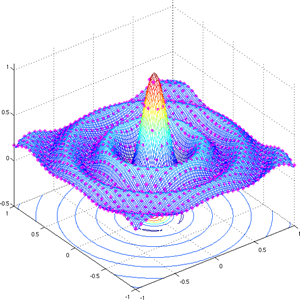
\includegraphics[scale=0.25]{../../img/sinc.PNG}}

\section{5.A.1}
\label{sec:org0e92b8d}


\begin{problem}
设\(T\in \mathcal{L}(V)\),并设\(U\)是\(V\)的子空间
\begin{enumerate}
\item 证明:若\(U\subset \mathrm{null} T\),则\(U\)在\(T\)下不变。
\item 证明:若\(\mathrm{range} T \subset U\),则\(U\)在\(T\)下不变。
\end{enumerate}
\end{problem}

\begin{answer}
\begin{enumerate}
\item \(\forall u\in U\) , \(Tu = 0\),因为\(U\)是\(V\)的子空间,所以\(0\in U\),所以\(Tu\in U\),所以\(U\)在\(T\)下不变
\item \(\forall u in U\),\(Tu \in \mathrm{range}T\)。因为\(\mathrm{range} T \subset U\),所以\(Tu \in U\) ,即\(U\)在\(T\)下不变。
\end{enumerate}
\end{answer}
\section{5.A.2}
\label{sec:org0897426}


\begin{problem}
设\(S,T\in \mathcal{L}(V)\)使得\(ST = TS\),证明\(\mathrm{null}S\)在\(T\)下不变。
\end{problem}

\begin{answer}
\(\forall u \in \mathrm{null}S\),则对\(ST = TS\)两边作用于\(u\),有\(STu = TSu = T(0) = 0\),显然有\(Tu \in \mathrm{null} S\)。
\end{answer}

\section{5.A.3}
\label{sec:org41e4929}


\begin{problem}
设\(S,T\in \mathcal{L}(V)\),使得\(ST = TS\),证明\(\mathrm{range} S\)在\(T\)下不变。
\end{problem}

\begin{answer}
设\(v \in \mathrm{range}S\),则\(\exists u\),使得\(Su = v\),所以\(STu = TSu = Tv\),即\(Tv\in \mathrm{range} S\)
\end{answer}

\section{5.A.4}
\label{sec:org5a91724}


\begin{problem}
设\(T\in \mathcal{L}(V)\)且\(U_{1},\ldots ,U_{m}\)是\(V\)的在\(T\)下不变的子空间。证明\(U_{1} + \ldots + U_{m}\)在\(T\)下不变。
\end{problem}

\begin{answer}
假设\(\forall u \in U_{1} + \ldots + U_{m}\),则\(\exists u_{1}\in U_{1},\ldots ,u_{m}\in U_{m}\),有\(u = u_{1} + \ldots + u_{m}\)。\(Tu = T(u_{1} + \ldots u_{m}) = Tu_{1} + \ldots + Tu_{m}\)。

因为\(Tu_{1} \in U_{1},\ldots ,Tu_{m} \in U_{m}\),所以\(Tu_{1} +\ldots + Tu_{m} \in Tu\)
\end{answer}

\section{5.A.5}
\label{sec:orgdead606}


\begin{problem}
设\(T\in \mathcal{L}(V)\),证明\(V\)的任意的一组在\(T\)下不变的子空间的交仍在\(T\)下不变。
\end{problem}

\begin{answer}
假设\(U_{1},\ldots ,U_{m}\)是\(T\)下的一组不变子空间,则对于\(U = U_{1}\cap \ldots \cap U_{m}\),假设\(u\in U\),则\(u\in U_{1},\ldots ,u\in U_{m}\),所以\(Tu \in U_{1},\ldots ,Tu \in U_{m}\),即\(Tu \in U_{1} \cap \ldots \cap U_{m}\)
\end{answer}
\section{5.A.6}
\label{sec:orgb75f46a}


\begin{problem}
证明或给出反例:若\(V\)是有限维的,\(U\)是\(V\)的子空间且在\(V\)的每个算子下不变,则\(U=\{0\}\)或者\(U=V\)
\end{problem}

\begin{answer}
我们用反证法证明这个命题是真命题。假设\(U\)是\(V\)的子空间,\(U\neq 0\)且\(U\neq V\),那么存在\(T\in \mathcal{L}(V)\)满足\(U\)在\(T\)下不是不变的。

假设\(U\)是\(V\)的子空间,\(U\neq 0\)且\(U\neq V\),对于\(u\in U\)且\(u\neq 0\)和\(w\in V, w\notin U\),扩展\(u\)为\(V\)的一个基\((u,v_{1},\ldots ,v_{n})\),定义:\[T(au+b_{1}v_{1} + \ldots + v_{n}v_{n}) = aw\]
因此\(Tu = w\)。因为\(u\in U\)但是\(w\notin U\),这表明\(U\)在\(T\)下不是不变的。
\end{answer}
\section{5.A.7}
\label{sec:org0442ebe}


\begin{problem}
定义\(T\in \mathcal{L}(\mathbf{R}^{2})\)为\(T(x,y) = (-3y,x)\),求\(T\)的本征值
\end{problem}

\begin{answer}
回忆一下本征值的定义。称数\(\lambda \in \mathbf{F}\)为\(T\)的本征值,若存在\(v\in V\)使得\(v\neq 0\)且\(Tv = \lambda v\)

我们假设\(\lambda\)是本征值,则有\((-3y,x) = \lambda (x,y)\),所以:
\begin{eqnarray}
\label{eq:1}
-3y&=& \lambda x \\
x&=& \lambda y
\end{eqnarray}
所以:
\begin{equation}
\label{eq:2}
-3y = \lambda^{2}y
\end{equation}
所以\(\lambda^{2} =  - 3\),这是不可能的。因为\(T\in \mathcal{L}(\mathbf{R}^{2})\)。
\end{answer}
\section{5.A.8}
\label{sec:org1e02090}


\begin{problem}
定义\(T\in \mathcal{L}(\mathbf{F}^{2})\)为\(T(w,z) = (z,w)\),求\(T\)的所有本征值和本证向量。
\end{problem}

\begin{answer}
根据本征值的定义。
\begin{eqnarray}
\label{eq:3}
(z,w)&=&\lambda (w,z) \\
\end{eqnarray}
所以\(\lambda = \pm 1\)。当\(\lambda = 1\)时,特征向量是\((w,w)\);当\(\lambda = -1\)时,特征向量是\((w,-w)\)
\end{answer}

\section{5.A.9}
\label{sec:org86d6610}


\begin{problem}
定义\(T\in \mathcal{L}(\mathbf{F}^{3})\)为\(T(z_{1},z_{2},z_{3}) = (2z_{2},0,5z_{3})\),求\(T\)的所有本征值和本证向量。
\end{problem}

\begin{answer}
根据本征值的定义。\[\lambda (z_{1},z_{2},z_{3}) = (2z_{2},0,5z_{3}) \]
\begin{eqnarray}
\label{eq:4}
\lambda z_{1}&=& 2z_{2}\\
\lambda z_{2}&=& 0 \\
\lambda z_{3}&=& 5z_{3}
\end{eqnarray}

所以当\(\lambda \neq 0\)我们可以得到:
\begin{eqnarray}
\label{eq:5}
\lambda &=& 5 \\
z_{2} &=&0 \\
z_{1} &=&0 \\
\end{eqnarray}
\(z_{3}\)是个自由变量,所以特征值是\(5\),特征向量是\((0,0,z_{3})\)

当\(\lambda =0\),我们可以得到:
\begin{eqnarray}
\label{eq:6}
z_{2}&=&0 \\
z_{3}&=&0 \\
\end{eqnarray}
\(z_{1}\)是个自由变量,所以特征值\(0\)对应的特征向量是\((z_{1},0,0)\)
\end{answer}

\section{5.A.10}
\label{sec:org29b6da2}


\begin{problem}
定义\(T\in \mathbf{F}^{n}\)为\(T(x_{1},x_{2},\ldots ,x_{n}) = (x_{1},2x_{2},3x_{3},\ldots ,nx_{n})\)
\begin{enumerate}
\item 求\(T\)的所有本征值和本证向量。
\item 求\(T\)的所有不变子空间。
\end{enumerate}
\end{problem}

\begin{answer}
\begin{enumerate}
\item 根据特征值的定义有:
\end{enumerate}
\begin{eqnarray}
\label{eq:7}
x_{1}&=&\lambda x_{1} \\
x_{2}&=&\lambda x_{2} \\
\vdots &=& \vdots \\
x_{n} &=&\lambda x_{n}
\end{eqnarray}

当\(\lambda = 0\)时,有\((x_{1},\ldots ,x_{n}) = (0,\ldots ,0)\),所以\(0\)不是\(T\)的特征值。当\(\lambda = 1\)时,我们有\((x_{1}\neq 0, 0,0,\ldots ,0)\)是\(T\)的特征向量,当\(\lambda = 2\)时,我们有\((0,x_{2}\neq 0, 0,0,\ldots ,0)\)是\(T\)的特征向量,依次类推,\(\lambda = n\)时,有\((0,0,\ldots ,x_{n}\neq 0)\)是\(T\)的特征向量。

\begin{enumerate}
\item 关于\(T\)的不变子空间,我们有\(n\)个特征向量对应的一维子空间肯定是\(T\)的不变子空间。
\end{enumerate}
\end{answer}
\section{5.A.11}
\label{sec:orgb58965b}


\begin{problem}
定义\(T: \mathcal{P}(\mathbf{R}) \rightarrow \mathcal{P}(\mathbf{R})\)为\(Tp = p^{'}\),求\(T\)的所有本征值和本证向量。
\end{problem}

\begin{answer}
本征值是对于\(T\in \mathcal{L}(V)\),存在\(\lambda\),对于非零的\(v\),有\(Tv = \lambda v\)。这个\(\lambda\)是本征值,\(v\)是对应的本证向量。

\(\mathcal{L}(\mathbf{R})\)是实数域上的多项式,则根据本征值的定义有\(\lambda \in \mathbf{R}\),且\(p\in \mathcal{L}(\mathbf{R})\)使得:
\begin{equation}
\label{eq:8}
\lambda p = p^{'}
\end{equation}
这个式子说明本证向量是\(\mathcal{P}(\mathbf{R})\)上的多项式,且满足其导数等于其本身的\(\lambda\)倍。指数函数具有这个性质,但是指数函数不是实数多项式。头疼,到底有没有本征值和本证多项式呢?如果\(\lambda = 0\)呢? \(\lambda p = 0\),又因为所有的常数导数都是零。所以\(\lambda = 0\),常数多项式是一对本征值和本证多项式。

一般情况下 \(\deg p^{'} < \deg p\),如果\(\lambda \neq 0\),有\(\deg \lambda q > \deg q^{'}\),矛盾。
\end{answer}
\section{5.A.12}
\label{sec:org3ed6287}


\begin{problem}
定义\(T\in \mathcal{L}( \mathcal{P}_{4}(\mathbf{R}))\)如下: 对所有\(x\in \mathbf{R}\)有\((Tp)(x) = xp^{'}(x)\),求\(T\)的所有本征值和本证向量。
\end{problem}

\begin{answer}
设有本征值为\(\lambda\),则有:
\begin{equation}
\label{eq:9}
\lambda p(x) = xp^{'}(x)
\end{equation}

我们知道\(p^{'}(x)\)比\(p(x)\)要低一个幂级,然后\(xp^{'}(x)\)又把幂提高一级,所以\(\lambda\)可以不是零。

对于\(p(x) = x^{n}\),\(p^{'}(x) = nx^{n-1}\),所以\(xp^{'}(x) = nx^{n}\).

定义\(q = a_{n}x^{n} + \ldots + a_{1}x + a_{0},a_{n}\neq 0\),所以:\[\lambda q =Tq = xq^{'}\]即,
\begin{equation}
\label{eq:10}
\lambda a_{n}x^{n} + \ldots + \lambda a_{1}x + \lambda a_{0} = na_{n}x^{n} + \ldots +  2a_{2}x^{2} + a_{1}x
\end{equation}

因为\(a_{n}\neq 0\),如果只考虑第一项,我们有\(\lambda = n\),然后\(a_{0} = a_{1} = \ldots = a_{n-1} = 0\),因此\(q = a_{n}x^{n}\) 所以\(T\)的特征值是\(0,1,\ldots\),各自对应的特征向量是\(\alpha x^{n}, \alpha\in \mathbf{R}\)
\end{answer}
\section{5.A.13}
\label{sec:orgf0fe82a}


\begin{problem}
设\(V\)是有限维的,\(T\in \mathcal{L}(V)\)且\(\lambda\in \mathbf{F}\),证明存在\(\alpha\in \mathbf{F}\)使得\(|\alpha - \lambda| < \frac{1}{1000}\) 且\((T-\alpha I)\)是可逆的。
\end{problem}

\begin{answer}
接触到这个题目,我拥有什么信息? \(\lambda\)不一定是特征值。这个题目有点奇怪。假设:
\begin{equation}
\label{eq:11}
|\alpha - \lambda| = \frac{1}{1000 + i}, i = 1,2,\ldots ,\dim V + 1
\end{equation}
又因为\(V\)至多有\(\dim V\)个特征值。多以在式 (\ref{eq:11})中一定有一个\(i\)使得\(\alpha_{i}\)不是\(T\)的特征值。

没有看出来这个题目有什么玄机。
\end{answer}

\section{5.A.14}
\label{sec:orgad9eac1}


\begin{problem}
设\(V = U\oplus W\),其中\(U\)和\(W\)均为\(V\)的非零子空间。定义\(P\in \mathcal{L}(V)\)如下:对\(u\in U\)和\(w\in W\)有\(P(u+w) = u\),求\(P\)的所有本征值和本证向量。
\end{problem}

\begin{answer}
根据本征值定义,\[\lambda(u+w) = u\] 所以有:\[(\lambda -1) u + \lambda w = 0\] 因为\(V = U\oplus W\)所以必须有\((\lambda -1)u = \lambda w = 0\)

\begin{enumerate}
\item 当\(u\neq 0\)时,\(\lambda = 1, w = 0\),对应的特征向量是\(u\in U, u\neq 0\).
\item 当\(w\neq 0\)时,\(\lambda = 0,\),此时\(u = 0\)。对应的特征向量是\(w\in W\)
\end{enumerate}
\end{answer}
\section{5.A.15}
\label{sec:orge2670ef}


\begin{problem}
设\(T\in \mathcal{L}(V)\),设\(S\in \mathcal{L}(V)\)是可逆的。

\begin{enumerate}
\item 证明\(T\)和\(S^{-1}TS\)有相同的本征值。
\item \(T\)的本证向量与\(S^{-1}TS\)的本证向量之间有什么关系?
\end{enumerate}
\end{problem}

\begin{answer}
对于第一个问题。假设\(T\)有特征值\(\lambda\)且\(\lambda\)对应的特征向量是\(v\)。因为\(S\)是可逆的,所以\(\exists u\in V\),使得\(Su= v\)。

所以\[Tv = \lambda v\],可以变成\[T(Su) = \lambda (Su)\] 即\[S^{-1}TS u = \lambda u\] 我们看到\(S^{-1}TS\)和\(T\)具有相同的特征值,但是特征向量不同。

对于第二个问题:我们在做第一个问题的时候就发现\(Su=v\),\(T\)的特征向量\(v\)和\(S^{-1}TS\)的特征向量\(u\)之间存在\(Su = v\)的关系。
\end{answer}
\section{5.A.16}
\label{sec:orgfe0bf76}


\begin{problem}
设\(V\)是复向量空间,\(T\in \mathcal{L}(V)\),\(T\)关于\(V\)的某个基的矩阵的元素均为实数。证明:若\(\lambda\)是\(T\)的本征值,则\(\bar{\lambda}\)也是\(T\)的本征值。
\end{problem}

\begin{answer}
不晓得我哪个知识点又欠缺了?这个问题不能顺利解决。

尽管这个命题在无穷维向量空间下也是真的。这里我们暂且只考虑有限维的情景。假设\(T\)相对于基\(e_{1},\ldots ,e_{n}\)的矩阵中所有元素都是实数,那么:
\[Te_{j} = \sum_{i=1}^{n}A_{i,k}e_{i}\]其中,\(A_{i,j}\in \mathbf{R}\),现在假设\(v\in V\)且可以表示为:
\[v = k_{1}e_{1} + \ldots + k_{n}e_{n}\]
是\(T\)的一个特征向量,对应的特征值是\(\lambda\)。
\[Tv = \lambda v\]
展开得到:
\[\lambda \sum_{i=1}^{n}k_{i}e_{i} = \sum_{i=1}^{n}k_{i}Te_{i} = \sum_{i=1}^{n}\sum_{j=1}^{n}k_{i}A_{j,i}e_{j}\]
对上式取共轭:
\[ \bar{\lambda} \sum_{i=1}^{n} \bar{k_{i}}e_{i} = \sum_{i=1}^{n}\bar{k_{i}}Te_{i} = \sum_{i=1}^{n}\sum_{j=1}^{n}\bar{k_{i}}A_{j,i}e_{j}\]
上式意味着:
\(T(\bar{k_{1}}e_{1} + \ldots + \bar{k_{n}}e_{n}) = \bar{\lambda}\sum_{i=1}^{n}\bar{k_{i}}e_{i}\)
即\(\lambda\)也是\(T\)的特征值。

注意上面证明过程中有个共轭的操作。
\end{answer}
\section{5.A.17}
\label{sec:org35c67e2}


\begin{problem}
给出一个没有(实)本征值的算子\(T\in \mathcal{L}(\mathbf{R}^{4})\)
\end{problem}

\begin{answer}
我们在例5.8中有一个\(T\in \mathcal{L}(\mathbf{R}^{2})\)上没有实本征值的算子\(T(w,z) = (-z,w)\),扩展该算子,有:
\[T\in \mathcal{L}(\mathbf{R}^{4}), T(x_{1},x_{2},x_{3},x_{4}) = (-x_{2},x_{1},-x_{4},x_{3})\]

这个问题的关键在于根据\(Tu = \lambda u\),找到一个\(\lambda^{2}\)是负数的方程。还是要根据定义来。
\end{answer}
\section{5.A.18}
\label{sec:orgd62ab5b}


\begin{problem}
定义\(T\in \mathcal{L}(\mathcal{C}^{\infty})\) 为\(T(z_{1},z_{2},\ldots ) = (0,z_{1},z_{2},\ldots ,)\),证明\(T\)没有本征值
\end{problem}

\begin{answer}
根据本征值的定义,假设有本征值\(\lambda\):
\[\lambda (0,z_{1},z_{2},\ldots ) = (z_{1},z_{2},\ldots ,)\]

显然有:
\begin{eqnarray}
\label{eq:12}
\lambda 0&=&z_{1} \\
\lambda z_{1}&=& z_{2} \\
&\vdots&
\end{eqnarray}
无论\(\lambda\)是否为零,都有\(0 = z_{1}=z_{2} = \ldots\)

而特征向量不能为零。因此不存在特征值\(\lambda\)。
\end{answer}
\section{5.A.19}
\label{sec:org361a5cd}


\begin{problem}
设\(n\)是正整数,定义\(T\in \mathcal{L}(\mathbf{F}^{n})\)为\(T(x_{1},\ldots ,x_{n}) = (x_{1}+\ldots +x_{n},\ldots ,x_{1}+\ldots +x_{n})\) 也就是说算子\(T\)对于标准基的矩阵的元素全是\(1\),求\(T\)的所有本征值和本证向量。
\end{problem}

\begin{answer}
利用特征值的定义, \(\lambda(x_{1},\ldots ,x_{n}) = (x_{1}+\ldots + x_{n},\ldots ,x_{1}+\ldots +x_{n})\),则有:
\begin{eqnarray}
\label{eq:13}
\lambda x_{1}&=&x_{1}+ \ldots + x_{n} \\
\lambda x_{2}&=&x_{1}+ \ldots + x_{n} \\
&\vdots& \\
\lambda x_{n}&=&x_{1}+ \ldots + x_{n}
\end{eqnarray}

把上面\(n\)个式子相加,则有\(\lambda = n\),此时\(x_{1} =x_{2}= \ldots =x_{n}\)。所以特征值为\(\lambda = n\),特征向量是\((x,\ldots ,x),x\in \mathbf{F}\)

当\(\lambda = 0\)时,所有满足\(x_{1} + \ldots + x_{n}=0\)的\((x_{1},\ldots ,x_{n})\)都是\(0\)对应的特征向量。
\end{answer}

\section{5.A.20}
\label{sec:org3e09c48}


\begin{problem}
定义向后移位算子\(T\in \mathcal{L}(\mathbf{F}^{\infty})\) 为\(T(z_{1},z_{2},z_{3},\ldots ) = (z_{2},z_{3},z_{4},\ldots )\)求\(T\)的特征向量和特征值。
\end{problem}

\begin{answer}
根据特征值定义:
\begin{eqnarray}
\label{eq:14}
z_{2} &=& \lambda z_{1} \\
z_{3} &=& \lambda z_{2} = \lambda^{2} z_{1} \\
&\vdots&
\end{eqnarray}
因此任何\(\lambda \in \mathbf{F}\)都是\(T\)的特征值,其对应的特征向量是\(\{(w,\lambda w, \lambda^{2} w,\ldots ): w\in \mathbf{F}\}\)

我们看到这个映射\(T\)对应的特征值有无穷多个,每个特征值对应的特征向量有无穷多个。
\end{answer}
\section{5.A.21}
\label{sec:org2765d77}


\begin{problem}
设\(T\in \mathcal{L}(V)\)是可逆的:
\begin{enumerate}
\item 设\(\lambda \in \mathbf{F},\lambda \neq 0\), 证明\(\lambda\)是\(T\)的本征值当且仅当\(\frac{1}{\lambda}\)是\(T^{-1}\)的本征值。
\item 证明\(T\)和\(T^{-1}\)有相同的本证向量。
\end{enumerate}
\end{problem}

\begin{answer}
\begin{enumerate}
\item 据本征值的定义,假设\(\lambda\)是\(T\)的本征值,\(v\)是对应的特征向量,则\[Tv = \lambda v\]对两边乘以\(T^{-1}\),则:\[v = \lambda T^{-1}v\] 进而有:\[T^{-1}v = \frac{1}{\lambda}\] 值得注意的是\(\lambda\)不可能是零,因为\(\lambda = 0\)则\(\lambda v = 0\),则\(Tv = 0\),因为\(T\)是可逆的,所以\(v = 0\),特征向量不能为零,矛盾。

\item 该命题的证明已经包含于命题1. 这个命题十个非常重要的结论。在以后会经常用到。
\end{enumerate}
\end{answer}

\section{5.A.22}
\label{sec:orgfee0a21}


\begin{problem}
设\(T\in \mathcal{L}(V)\)且存在\(V\)中的非零向量\(v\)和\(w\)使得\(Tv = 3w\),且\(Tw = 3v\),证明\(3\)或者\(-3\)是\(T\)的特征值。
\end{problem}

\begin{answer}
因为:
\begin{eqnarray}
\label{eq:15}
Tv&=&3w \\
Tw&=&3v
\end{eqnarray}
两式相加:\[T(v+w) = 3(w+v)\]
两式相减:\(T(v-w) = 3(w-v) = -3(v-w)\)
当\(v=w\)时,\(3\)是\(T\)的特征值,对应的特征向量为\(2v\)。
当\(v=-w\)时,\(-3\)是\(T\)的特征值,对应的特征向量是\(-2w\)。
当\(v\neq w, v\neq -w\)时,\(3\)和\(-3\)都是\(T\)的特征值,对应的特征向量是\(v+w\)和\(v-w\)
\end{answer}

\section{5.A.23}
\label{sec:org7b0e966}


\begin{problem}
设\(V\)是有限维的,且\(S,T\in \mathcal{L}(V)\)。证明\(ST\)和\(TS\)有相同的本征值。
\end{problem}

\begin{answer}
假设\(\alpha\)是\(ST\)的特征值,对应的特征向量是\(u\);我们要证明\(\lambda\)是\(TS\)的特征值。
\begin{eqnarray}
\label{eq:17}
(TS)(Tu)&=&T(ST)u \\
&=&T(\lambda u) \\
&=&\lambda (Tu)
\end{eqnarray}
当\(Tu\neq 0\)时,\(Tu\)就是\(TS\)的特征值。

当\(Tu=0\),那么\(\lambda = 0\) (因为\(STu = \lambda u\)),所以\(T\)不是可逆的,继而\(TS\)也不是可逆的。\(TS\)不是可逆的,就有\(u\in V\)使得\(TS u = 0 = 0u\),即\(0\)是\(TS\)的特征值。

我们有不管\(Tu\)是否为零,\(\lambda\)都是其\(TS\)特征值。
\end{answer}
\section{5.A.24}
\label{sec:orgd5da89d}


\begin{problem}
设\(A\)是元素属于\(\mathbf{F}\)的\(n\times n\)矩阵。定义\(T\in \mathcal{L}(\mathbf{F}^{n})\)为\(Tx = Ax\),这里\(\mathbf{F}^{n}\)中的元素视为\(n\times 1\)的列向量。
\begin{enumerate}
\item 设\(A\)的每行元素之和都是1,证明\(1\)是\(T\)的本征值。
\item 设\(A\)的每列元素之和都是1,证明\(1\)是\(T\)的本征值。
\end{enumerate}
\end{problem}

\begin{answer}
因为\(Tx = Ax\);
\begin{eqnarray}
\label{eq:18}
Ax =
\begin{bmatrix}
a_{11}x_{1} + a_{12}x_{2} + \ldots + a_{1n}x_{n} \\
a_{21}x_{1} + a_{22}x_{2} + \ldots + a_{2n}x_{n} \\
\vdots \\
a_{n1}x_{1} + a_{n2}x_{2} + \ldots + a_{nn}x_{n}
\end{bmatrix}
\end{eqnarray}

注意到当\(x_{1}=x_{2}=\ldots =x_{n}=\frac{1}{n}\)时,有:
\begin{equation}
\label{eq:19}
Ax = x
\end{equation}
即\(1\)是\(T\)的本征值。我们可以看到针对特征值\(1\),\(T\)有特征向量\[\{(x_{1},x_{2},\ldots ,x_{n}: x_{1} = x_{2} = \ldots = x_{n} \neq 0)\}\]
\end{answer}
\begin{answer}
对于第二个问题:我们有:
\begin{equation}
\label{eq:20}
(T-I)
\begin{bmatrix}
x_{1} \\  \vdots \\ x_{n}
\end{bmatrix}
=
\begin{bmatrix}
\sum_{i=1}^{n}a_{1i}x_{i} - x_{1} \\
\vdots \\
\sum_{i=1}^{n}a_{ni}x_{i} - x_{n}
\end{bmatrix}
=
\begin{bmatrix}
y_{1} \\
\vdots \\
y_{n}
\end{bmatrix}
\end{equation}
显然\(T-I\)的值域不是\(\mathbf{F}^{n}\),因此\(T-I\)不是双射,即\(T-I\)不是单射,所以存在\(u\in \mathrm{null}(T-I),u\neq \mathbf{0}\),使得:\[(T-I)u = 0\]
\end{answer}
\section{5.A.25}
\label{sec:org799ea63}


\begin{problem}
设\(T\in \mathcal{L}(V)\)且\(u\)和\(v\)均为\(T\)的本证向量使得\(u+v\)也是\(T\)的本证向量。证明\(u\)和\(v\)是\(T\)的同一本征值的本证向量。
\end{problem}

\begin{answer}
根据5.10,不同本征值的特征向量是线性无关的,很容易可以证明。
\end{answer}

\section{5.A.26}
\label{sec:org416c0f9}


\begin{problem}
设\(T\in \mathcal{L}(V)\)使得\(V\)中的每个非零向量都是\(T\)的本征向量。证明\(T\)是恒等算子的标量倍。
\end{problem}

\begin{answer}
如果\(\forall v\in V, \exists a_{v}\in \mathbf{F}, \mathrm{s.t.} \quad Tv = a_{v} v\)。因为\(T0 = 0\),我们可以选\(a_{0}\)为任意的数。对于\(v\in V\backslash \{0\}\) 我们证明\(a_{v}\)由\(Tv = a_{v}v\)唯一确定。

为了证明\(T\)是恒等算子的标量倍,我们必须证明对于所有的\(v\in V\backslash \{0\}\),\(a_{v}\)不变的。特别的,假设\(v,w \in V\backslash \{0\}\),我们证明\(a_{v}=a_{w}\)首先考虑\(v,w\)线性相关,那么\(\exists~b, \mathrm{s.t.}\quad w=bv\),所以:
\begin{eqnarray}
\label{eq:21}
a_{w}w&=&Tw \\
&=&Tbv \\
&=&bTv \\
&=&ba_{v}v \\
&=&a_{v}b_{v}\\
&=&a_{v}w
\end{eqnarray}
所以\(a_{v} = a_{w}\)

另外考虑\(v,w\)是线性独立的,则:
\begin{eqnarray}
\label{eq:23}
a_{v+w}(v+w)&=&T(v + w) \\
&=&a_{v}v + a_{w}w
\end{eqnarray}
这意味着:\((a_{v+w} - a_{v})v + (a_{v+w} - a_{w})w = 0\)
\begin{eqnarray}
\label{eq:24}
a_{v+w}&=&a_{v} \\
a_{v+w}&=&a_{w}
\end{eqnarray}
即\(a_{v}=a_{w}\).

综上,命题得证。
\end{answer}
\section{5.A.27}
\label{sec:orgc577bb2}


\begin{problem}
设\(V\)是有限维的,\(T\in \mathcal{L}(V)\)使得\(V\)的每个\(\dim V -1\)维子空间都在\(T\)下不变。证明\(T\)是恒等算子的标量倍。
\end{problem}

\begin{answer}
利用上题的结论,假设\(T\)不是恒等算子的标量倍,则一定存在\(u\)不是\(T\)的特征向量,则\(Tu\)和\(u\)是线性独立的。我们把\(u,Tu\)扩展为\(V\)的一个基,\((u,Tu,v_{1},\ldots ,v_{n})\),令
\[U = \mathrm{span}(u,u_{1},\ldots ,u_{n})\]
显然,\(\dim U = \dim V -1\)。我们可以看到\(U\)在\(T\)下不是不变的因为\(Tu\notin U\)。矛盾。因此\(T\)一定是恒等算子的标量倍。
\end{answer}

\section{5.A.28}
\label{sec:org0b4a9ab}


\begin{problem}
设\(V\)是有限维的,\(\dim V \geq 3\)且\(T\in \mathcal{L}(V)\)使得\(V\)的每个二维子空间都在\(T\)下不变。证明\(T\)是恒等算子的标量倍。
\end{problem}

\begin{answer}

\end{answer}
\section{5.A.29}
\label{sec:orgdc94855}


\begin{problem}
设\(T\in \mathcal{L}(V)\)且\(\dim \mathrm{range}(T) = k\),证明\(T\)至多有\(k+1\)个不同的特征值。
\end{problem}

\begin{answer}
\[\dim V = \dim \mathrm{null}T + \dim \mathrm{range}T\]
假设\(\mathrm{null}T \neq \{0\}\),\(\exists u\in \mathrm{null}T, u\neq 0, \mathrm{s.t.} \quad Tu = 0\),则\(0\)是\(T\)的一个特征值.

假设\(T\)有\(m\)个互不相同的特征值,\(\lambda_{1},\ldots ,\lambda_{m}\),并且\(v_{1},\ldots ,v_{m}\)是这些特征值对应的特征向量。则有如果\(\lambda_{i}\neq 0\),则:
\begin{equation}
\label{eq:25}
T(v_{j}/\lambda_{j})= v_{j}
\end{equation}
因为\(\lambda_{j}\)中最多有一个为\(0\),这个零是我们之前做的假设导致的。那么也就是说\(\lambda_{j}\)中至少有\(m-1\)个向量在\(\mathrm{range}(T)\)中。这些向量是线性无关的,则:
\begin{equation}
\label{eq:26}
m - 1 \leq \dim \mathrm{range}(T) = k
\end{equation}
因此\(m\leq k+1\),证闭。
\end{answer}
\section{5.A.30}
\label{sec:org901b0ee}


\begin{problem}
设\(T\in \mathcal{L}(\mathbf{R}^{3})\),且\(4,5,\sqrt{7}\)是\(T\)的本征值,证明存在\(x\in \mathbf{R}^{3}\)使得\(Tx - 9x = (4,5,\sqrt{7})\)
\end{problem}

\begin{answer}
已知,\(\dim \mathbf{R}^{3} = 3\),且\(T\)有三个互不相同的特征值,则其对应的特征向量是线性无关的。这说明\(9\)肯定不是\(T\)的特征值。因此\(T-9I\)是满射。因此\(\exists x\in \mathbf{R}^{3}, \mathrm{s.t.}\quad (T-9I)x = (4,5,\sqrt{7})\),即\(Tx - 9x = (4,5,\sqrt{7})\)
\end{answer}
\section{5.A.31}
\label{sec:org85840fb}


\begin{problem}
设\(V\)是有限维的且\(v_{1},\ldots ,v_{m}\)是\(V\)中的一组向量。证明\(v_{1},\ldots ,v_{m}\)线性无关当且仅当存在\(T\in \mathcal{L}(V)\),使得\(v_{1},\ldots ,v_{m}\)是\(T\)的相应于不同特征值的特征向量。
\end{problem}

\begin{answer}
首先,我们知道假设\(v_{1},\ldots ,v_{m}\)是\(T\in \mathcal{L}(V)\)的相应于不同特征值的特征向量,则\(v_{1},\ldots ,v_{m}\)是线性无关的。

然后我们证明另外一个方面。假设\(v_{1},\ldots ,v_{m}\)是线性无关的,则\(v_{1},\ldots ,v_{m}\)可以扩展为\(V\)的一组基\(v_{1},\ldots ,v_{m},v_{m+1},\ldots ,v_{n}\),定义\(T\in \mathcal{L}(V)\)为:
\begin{equation}
\label{eq:28}
Tv_{i} = iv_{i},i = 1,\ldots ,n
\end{equation}
因此,\(v_{1},\ldots ,v_{n}\)是\(T\)的对应于\(1,\ldots ,n\)的特征向量。
\end{answer}
\section{5.A.32}
\label{sec:orge27a986}


\begin{problem}
设\(\lambda_{1},\ldots ,\lambda_{m}\)是一组互异实数。证明在由\(\mathbf{R}\)上的实值函数构成的向量空间中,组\(e^{\lambda_{1}x},\ldots ,e^{\lambda_{n}x}\)线性无关。
\end{problem}

\begin{answer}
定义:\[Tf = f^{'}\]则有:
\[Te^{\lambda_{i}x} = \lambda_{i}e^{\lambda_{i}x}\] 因此\(\lambda_{i}\)是\(T\)的对应于\(e^{\lambda_{i}x}\)的特征值。因为\(\lambda_{i}\)各不相同,所以\(e^{\lambda_{i}x},\forall i\)是线性独立的。
\end{answer}
\end{document}
